\subsection{Experiments}
\label{sub:Experiments}
In order to determine the reliability of the hardware, several experiments were conducted on the PIR sensor. The tests were all based on results found in the data sheet for the hardware. The main purpose of these tests is to determine the properties of the batch of sensor used in project compared to the properties given in the data sheets\cite{datasheet_pir1}\cite{datasheet_pir2}.
\\\\
The four tests are defined as follows:

\begin{enumerate}
  \item Sensitivity Test
  \item Angle Test
  \item Distance Test
  \item Holding Time Test
\end{enumerate}

\subsection{The Setup}
\label{subs:The Setup}
As mentioned, the setup for all the experiments is the same, to ensure
consistency of the results, by reducing variables that affect the results, as
much as possible. The PIR sensor is placed, surrounded by walls, with no unwanted
moving objects within its field of view. In order to ensure that the results are
as precise as possible, all four tests are carried out at the same exact place,
but the methods of the individual tests differ. The PIR sensor is placed in a
certain height and a fixed position during the tests.

\subsubsection{Sensitivity}
\label{par:Sensitivity}

\paragraph{Hypothesis}
\label{subp:SenHypothesis}
According to the data sheet the PIR sensor will be too sensitive if the distance potentiometer is rotated counter-clockwise.
The sensor should get so sensitive that the PIR sensor would be triggered by the atmosphere even
if no moving object is existing\cite{datasheet_pir1}.
\paragraph{Test Procedure}
\label{subp:SenTest Procedure}
The PIR sensor is configured with the distance potentiometer rotated
counter-clockwise, as far as possible.
After the sensor is configured every object that can affect the sensor is
removed and the sensor is observed for 30 seconds.
The observation is to determine whether the sensor will detect objects, that it is not
supposed to detect, and how sensitive the sensor really is.
\paragraph{Results}
\label{subp:SenResults}

At the most sensitive setting, nothing was triggered by atmospheric noise. Just
to be sure, the sensor was tested at the least sensitive setting; nothing was
detected, as expected.

\paragraph{Partial Conclusion}
\label{subp:SenPartial Conclusion}

According to our tests, the atmospheric noise was not detectable at the highest
sensitivity setting.

\subsubsection{Angle}
\label{par:Angle}

\paragraph{Hypothesis}
\label{subp:AngHypothesis}
According to the data sheet of the PIR sensor,
the sensor has a detecting angle of 120 degrees.
The sensor should, according to the data sheet not detect any angle above 120 degrees.

\paragraph{Test Procedure}
\label{subp:AngTest Procedure}
The sensor is placed in a certain position and detecting angle is measured equivalent to
the specified angle found in the data sheet.
For the sake of explanation, let the angle above 120 degree be the grey zone and
the detecting area, that is within the 120 degrees, the white zone.
A moving object is placed in the grey zone and slowly moves into the white zone.
The PIR sensor should be triggered, when the moving object enters the white zone in order
to work as specified in the hardware specifications.
The zone of the moving object and PIR sensor is observed accordingly
and thereby the actual detecting angle is determined.

The test is performed three times on each side at the highest sensitivity of the sensor for consistency.

\paragraph{Results}
\label{subp:AngResults}

The data results can be seen in \cref{tab:pir_angle}. A plot of this data can be
seen in \cref{fig:pir_angle}.

\begin{figure}[htbp]
\centering
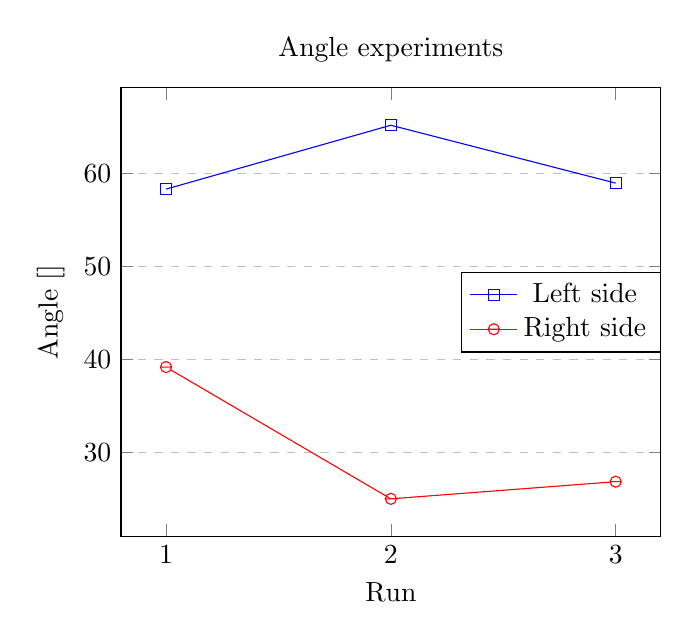
\begin{tikzpicture}
\begin{axis}[
    title={Angle experiments},
    xlabel={Run},
    ylabel={Angle [$\si{\degree}$]},
    xtick={1,2,3},
    legend style={at={(1,0.5)},anchor=east},
    ymajorgrids=true,
    grid style=dashed,
]
\addplot[
    color=blue,
    mark=square,
    ]
    coordinates {
    (1,58.3136)
    (2,65.1905)
    (3,58.9582)
    };
\addlegendentry{Left side}
% asd
\addplot[
    color=red,
    mark=halfcircle,
    ]
    coordinates {
    (1,39.1605)
    (2,24.9812)
    (3,26.8278)
    };
\addlegendentry{Right side}
\end{axis}
\end{tikzpicture}
\caption[Angle experiment]{Plot of angle experiment}\label{fig:pir_angle}
\end{figure}

\begin{table}[htbp]
\centering
\begin{tabular}{@{}llll@{}}
\toprule
Run & x [cm] & y [cm] & angle [deg] \\ \midrule
1 (left) & 81 & 50 & 58.3136 \\
1 (right) & 79 & 97 & 39.1605  \\ \midrule
2 (left) & 106 & 49 & 65.1905 \\
2 (right) & 82 & 176 & 24.9812 \\ \midrule
3 (left) & 108 & 65 & 58.9582 \\
3 (right) & 88 & 174 & 26.8278 \\ \bottomrule
\end{tabular}
\caption[Angle experiment results]{Results of angle experiments. The x and y columns represent the width and height
  distance from the sensor to the detected person. The angle values are
  calculated by $\arctan (x,y) * \frac{180}{\pi}$}
\label{tab:pir_angle}
\end{table}

\paragraph{Partial Conclusion}
\label{subp:AngPartial_conclusion}

According to the hypothesis, the sensor should detect motion in an angle of 120 degrees. Our results show that the left side of the sensor is quite correct, while the other side of the sensor is not very close to 60 $\si{\degree}$.

\subsubsection{Distance}

\paragraph{Hypothesis}

According to the data sheet, the sensor can measure motion from 10 centimetres to
6 meters.

\paragraph{Test procedure}

The sensitivity setting of the sensor essentially controls the distance. First,
the sensitivity is set to the lowest sensitivity. At that sensitivity, the
sensor should detect motion at a range of 10 centimetres, according to the above
hypothesis.

The sensor is measured by the test conductor approaching the sensor while
waving. Once the sensor detects the motion, the distance from the test conductor
to the sensor is measured. This is done three times to check for consistency. The sensitivity is then upped one unit on the sensor,
and the test conductor measures the distance for the new sensitivity.

\paragraph{Results}

A plot of the results can be seen in \cref{fig:pir_distance}.

\begin{figure}[htbp]
\centering
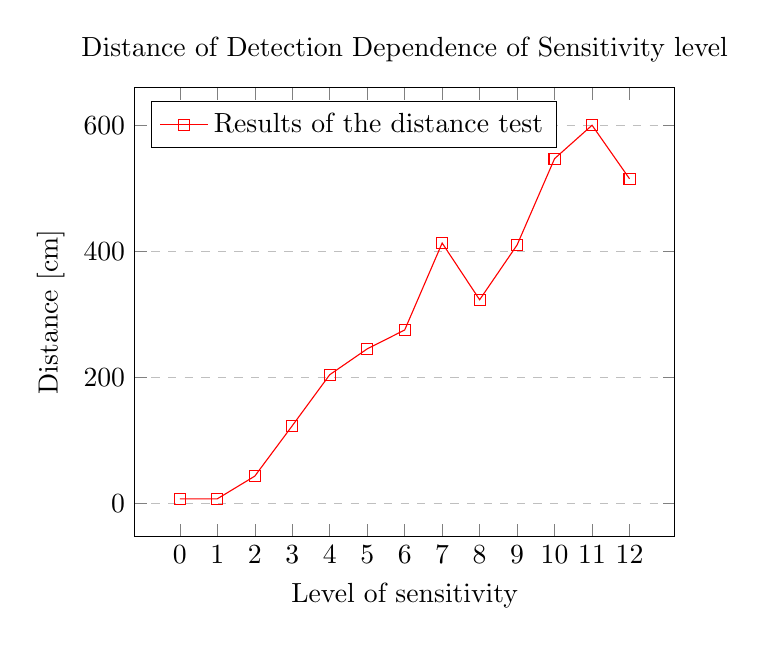
\begin{tikzpicture}
\begin{axis}[
    title={Distance of Detection Dependence of Sensitivity level},
    xlabel={Level of sensitivity},
    ylabel={Distance [cm]},
    %xmin=0, xmax=12,
    %ymin=0, ymax=120,
    xtick={0,1,2,3,4,5,6,7,8,9,10,11,12},
    %ytick={0,20,40,60,80,100,120},
    legend pos=north west,
    ymajorgrids=true,
    grid style=dashed,
]

\addplot[
    color=red,
    mark=square,
    ]
    coordinates {
    (0,7)(1,7)(2,43)(3,123)(4,204)(5,245)(6,275)(7,413)(8,323)(9,410)(10,547)(11,600)(12,515)
    };
    \legend{Results of the distance test}

\end{axis}
\end{tikzpicture}
\caption[Distance experiment]{Plot of distance experiment}\label{fig:pir_distance}
\end{figure}

\paragraph{Partial conclusion}
The results indicate that there is a correlation between the sensitivity and the detecting distance.
However the sensor behaved unpredictably at sensitivity levels 7 and 8.
Furthermore the sensor acted strange at sensitivity levels 3, 4 and 5 by detecting something it was not supposed to detect.
The maximum range seems to be 6 meters as stated in the data sheet.
Strangely enough the sensor only detected motion 5 meters away at the highest
sensitivity level.

\subsubsection{Holding time}

\paragraph{Hypothesis}

According to the data sheet, the sensor has a holding time of 1 second to 25 seconds.

\paragraph{Test procedure}

In this experiment, the sensor is set in the non-retriggerable setting, so the holding time is not extended on additional motion.

First, the sensor is adjusted to have the maximum holding time of 25 seconds,
according to the above hypothesis. This is then tested by triggering the sensor
and starting a stopwatch simultaneously. When the sensor stops signalling, the
stopwatch is stopped and the actual holding time noted. This is done three times
for each setting of holding time to check for consistency.

For the next iteration of the experiment, the holding time potentiometer on the sensor
is rotated one unit, decreasing the holding time.

\paragraph{Results}

A plot of the results can be seen in \cref{fig:pir_delay}.

\begin{figure}[htbp]
\centering
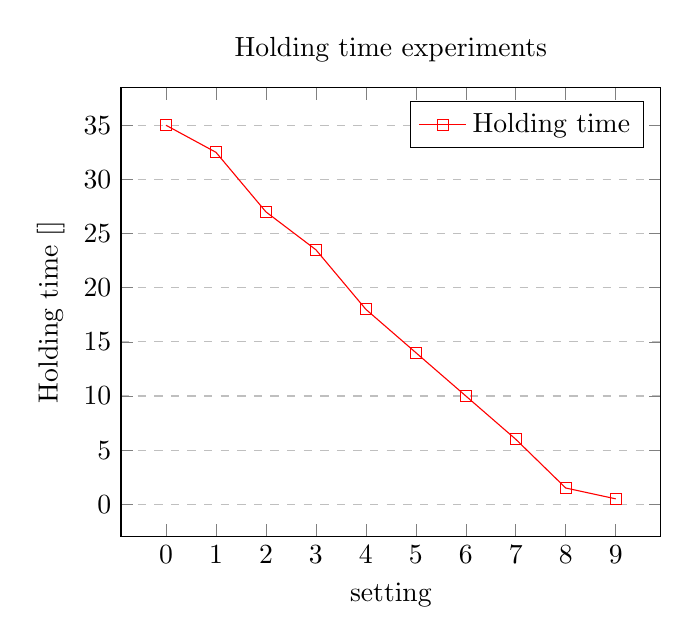
\begin{tikzpicture}
\begin{axis}[
    title={Holding time experiments},
    xlabel={setting},
    ylabel={Holding time [$\si{\second}$]},
    xtick={0,1,...,9},
    ytick={0,5,...,40},
    legend pos= north east,
    ymajorgrids=true,
    grid style=dashed,
]
\addplot[
    color=red,
    mark=square,
    ]
    coordinates {
    (0,35)
    (1,32.5)
    (2,27)
    (3,23.5)
    (4,18)
    (5,14)
    (6,10)
    (7,6)
    (8,1.5)
    (9,0.5)
    };
\addlegendentry{Holding time}
\end{axis}
\end{tikzpicture}
\caption[Holding experiment]{Plot of holding time experiment. On the x axis number representation of potentiometer, ranging from 0 with longest holding time to 9 with shortest holding time. On the y axis the holding time in seconds are shown.}\label{fig:pir_delay}
\end{figure}

\paragraph{Partial conclusion}

The hypothesis is incorrect. The maximum holding time was recorded to be around 35 seconds that is a deviation by more than 30\%.
However, the minimum holding time was very close to the value described in the hypothesis.
